\paragraph{}Tras haber solicitado el presupuesto mediante el botón \textit{\textbf{''Realizar Pedido''}}, el usuario es redirigido automáticamente a la función de imprimir de su navegador para poder imprimir el pedido que se genera en formato PDF. En el que se muestra toda la información relativa al pedido que se acaba de realizar. Un pedido está compuesto por los siguientes elementos:

\begin{itemize}
	\item \textbf{Tabla de artículos solicitados:} En esta tabla se refleja el número de unidades de cada artículo, las referencias, el precio por unidad de cada uno, el precio subtotal para cada referencia y el precio final del pedido.
	
	\item \textbf{Datos del cliente:} Listado con los datos introducidos por el cliente que permiten tanto identificar al cliente como contactar con él si fuese necesario.
\end{itemize}

\begin{figure}[h!]
	\centering
	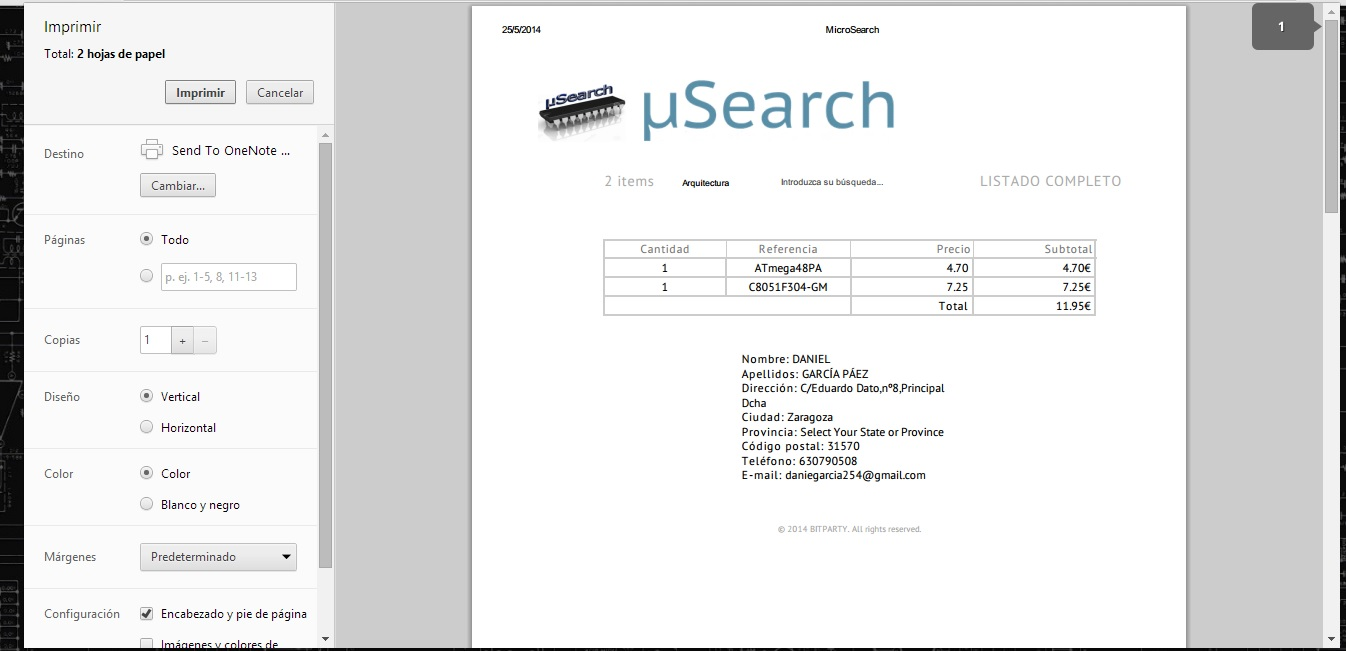
\includegraphics[width=0.85\textwidth]{img/pedido}
	\caption{Pedido generado en PDF.}
	\label{fig:pedido}
\end{figure}

\paragraph{} Tras imprimir el pedido, o cancelar su impresión, al usaurio se le muestra un mensaje de agradecimiento por su compra; pudiendo de nuevo navegar libremente por el catálogo y realizar más pedidos.